\documentclass[11pt]{article}
\newcommand{\doctype}{Preprint}
\newcommand{\docversion}{v0.02.002}
\newcommand{\docdate}{2 November 2026}
\newcommand{\versiondoi}{10.5281/zenodo.23899142}
\newcommand{\conceptdoi}{10.5281/zenodo.23875071}
\newcommand{\docrepo}{github.com/fsantibanezleal/CAOS\_SoftQP}
\newcommand{\docscope}{side-specific and directional peak penalties}
\newcommand{\shorttitle}{Original-row proximal updates}
% Presentation derived from the canonical CAOS Research foundational article.
\usepackage[T1]{fontenc}
\usepackage[utf8]{inputenc}
\usepackage{lmodern,microtype}
\usepackage[margin=1.1in,headheight=15pt]{geometry}
\usepackage{amsmath,amssymb,amsthm}
\usepackage{booktabs,array,tabularx,longtable,graphicx}
\usepackage{algorithm,algpseudocode}
\usepackage{xcolor,xurl}
\definecolor{linknavy}{RGB}{25,55,125}
\usepackage[colorlinks=true,linkcolor=linknavy,citecolor=linknavy,urlcolor=linknavy]{hyperref}
\usepackage{orcidlink}
\usepackage{fancyhdr}
\newtheorem{theorem}{Theorem}[section]
\newtheorem{proposition}[theorem]{Proposition}
\newtheorem{lemma}[theorem]{Lemma}
\theoremstyle{definition}
\newtheorem{definition}[theorem]{Definition}
\theoremstyle{remark}
\newtheorem{remark}[theorem]{Remark}
\DeclareMathOperator{\prox}{prox}
\DeclareMathOperator{\diag}{diag}
\DeclareMathOperator{\median}{median}
\DeclareMathOperator{\argmin}{argmin}
\newcommand{\R}{\mathbb{R}}
\newcommand{\pos}[1]{\left(#1\right)_{+}}
\newcommand{\norm}[1]{\left\lVert#1\right\rVert_{\infty}}
\newcommand{\headerblock}{%
\begin{center}
\fbox{\parbox{0.94\textwidth}{\small\raggedright
\textbf{\doctype} \quad$\cdot$\quad \docversion, \docdate \quad$\cdot$\quad Licence CC BY 4.0\\[2pt]
CAOS Research programme \quad$\cdot$\quad \docscope\\[2pt]
Version DOI \href{https://doi.org/\versiondoi}{\texttt{\versiondoi}}\\[2pt] % voice-ok: required page-one header identity, not body narrative
Concept DOI (always latest) \href{https://doi.org/\conceptdoi}{\texttt{\conceptdoi}}\\[2pt] % voice-ok: required page-one header identity, not body narrative
Not peer reviewed. Source code, data and computational records:
\href{https://\docrepo}{\texttt{\docrepo}}
}}
\end{center}
\vspace{4pt}}
\pagestyle{fancy}
\fancyhf{}
\fancyhead[L]{\small CAOS Research \doctype}
\fancyhead[R]{\small \shorttitle\ \textperiodcentered\ \docversion}
\fancyfoot[C]{\small \thepage}
\renewcommand{\headrulewidth}{0.4pt}
\fancypagestyle{plain}{\fancyhf{}\fancyfoot[C]{\small \thepage}\renewcommand{\headrulewidth}{0pt}}
\setlength{\emergencystretch}{1.5em}

% Numeric export from the reviewed summary; no new inference.
\newcommand{\PrimaryEstimate}{-212.449875}
\newcommand{\PrimaryLower}{-225.336618}
\newcommand{\PrimaryUpper}{-192.873759}
\newcommand{\PrimaryFailed}{9}
\newcommand{\PrimaryPopulation}{144}
\newcommand{\SummaryDigest}{c82bf30bb53c7c10d464fc446bd2b99ee774b581dbe3f4dced86194e1fe54c6d}
\newcommand{\DevelopmentAccepted}{879}
\newcommand{\DevelopmentAccuracyRejected}{0}
\newcommand{\DevelopmentIncompatible}{396}
\newcommand{\DevelopmentOracleFailed}{21}
\newcommand{\DevelopmentTimeout}{0}
\newcommand{\HeldoutAccepted}{2587}
\newcommand{\HeldoutAccuracyRejected}{6}
\newcommand{\HeldoutIncompatible}{1188}
\newcommand{\HeldoutOracleFailed}{105}
\newcommand{\HeldoutTimeout}{2}
\newcommand{\RobustnessAccepted}{201}
\newcommand{\RobustnessAccuracyRejected}{6}
\newcommand{\RobustnessIncompatible}{135}
\newcommand{\RobustnessOracleFailed}{144}
\newcommand{\RobustnessTimeout}{0}

% Exact exported original-study summary; no inferential recomputation.
\newcommand{\OriginalEstimate}{0.499839}
\newcommand{\OriginalLower}{-3.291967}
\newcommand{\OriginalUpper}{3.944835}
\newcommand{\OriginalPairs}{168}

\title{Original-Row Proximal Updates for Side-Specific and Directional Peak Penalties: Two Negative Timing Studies}
\author{Felipe Santib\'a\~nez-Leal\,\orcidlink{0000-0002-0150-3246}\\
\small CAOS Research program, \texttt{github.com/fsantibanezleal/CAOS\_SoftQP}}
\date{\docdate}
\hypersetup{pdftitle={Original-Row Proximal Updates for Side-Specific and Directional Peak Penalties: Two Negative Timing Studies},pdfauthor={Felipe Santibáñez-Leal}}
\begin{document}
\maketitle
\thispagestyle{plain}
\headerblock
\begin{abstract}
Original-row proximal updates can represent selected soft interval penalties
without adding explicit departure variables to a quadratic program's principal
system. We derive a side-specific separable linear--quadratic update and a
directional disjoint group-peak update in a fixed positive diagonal metric.
The grouped construction follows a box-residual identity under coordinate
contractions and reduces its proximal operation to a weighted scalar threshold.
Exact lifting, directional row splitting and compact epigraphs already express
the same objectives; no expressibility or algorithmic-priority claim is made.
We evaluate the two implementations in separate registered synthetic studies.
The first contains 456 instances and 168 held-out accepted pairs: median
relative cold end-to-end reduction \OriginalEstimate\%, with 95\% seed-cluster
limits \OriginalLower\% and \OriginalUpper\%. The second contains 210
repeated-forecast instances, with a 144-member held-out primary score of
\PrimaryEstimate\%, limits \PrimaryLower\% and \PrimaryUpper\%, and
\PrimaryFailed{} retained failed pairs. Neither predicted ten-percent timing
improvement is established. Original-space objective, hard-row and dual
checks distinguish mathematical equivalence from computational cost. Retained
formulation, conditioning and workspace comparisons characterize components
without asserting an unperformed causal ablation. The results show that fewer
principal variables or rows do not by themselves establish a faster complete
optimization operation on these tested populations.
\end{abstract}
\section{Introduction}\label{sec:introduction}
Soft interval constraints specify a price for violating a preference while
leaving selected physical limits immutable. In predictive control, a preferred
state range and an actuator capacity are not interchangeable constraints.
In energy scheduling, an upper grid departure and a lower comfort departure
can have different units and consequences. The numerical problem must state
which rows may yield and which objective measures that choice before a solver
comparison has a definite meaning. Convex quadratic objectives with such
interval penalties provide a useful, transparent setting for that analysis.

An ordinary slack lift expresses many of these prices exactly, but enlarges
the mathematical system. Generalized slack projections replace selected slack
variables with proximal row operations and can preserve the original principal
dimensions~\cite{gsp,lew}. That observation motivates a computational hypothesis:
an original-row implementation might reduce the cost of a complete optimization
operation. It does not prove the hypothesis. A proximal operation can itself
be expensive, sparse fill depends on more than dimension, and preparation,
validation and recovery contribute to the measured operation.

We study two related original-row updates. The first applies separate
nonnegative linear--quadratic prices to lower and upper interval departures.
Its scalar proximal minimizer follows from exterior quadratic stationarity
and endpoint subgradient conditions. The second prices directional disjoint
group peaks. A box-residual identity under coordinate contractions reduces
its positive diagonal-metric proximal operation to a weighted scalar threshold.
We state the precise fixed-metric and relaxation scope, preserve hard rows
separately, and test outputs in original physical coordinates. Existing
side-weighted active-set formulations, directional row splitting and compact
epigraphs already express the same objectives~\cite{daqp,gsp}. Consequently,
neither unequal side costs nor directional expressibility is a priority claim.

The two computational evaluations are separately registered synthetic studies.
The original study contains 456 instances, with 168 primary paired observations
from 24 distinct held-out problems and seven repetitions across six seed clusters.
Its median cold end-to-end reduction is \OriginalEstimate\%, with 95\% limits
\OriginalLower\% and \OriginalUpper\%. The grouped study contains 210 instances
and a complete 144-instance held-out population. Its primary score is
\PrimaryEstimate\%, with limits \PrimaryLower\% and \PrimaryUpper\%, including
\PrimaryFailed{} failed pairs. Both predicted 10\% improvements are unestablished.
These findings concern different measurement boundaries and cannot be pooled
into a new favorable estimator.

The contribution is a derivation and implementation analysis with explicit
negative computational evidence. We provide the side-specific proximal formula,
the contraction-based box reduction, the directional threshold and conjugate,
and the fixed-metric splitting conditions. We compare exact objective-matched
references and retain compatibility limits, unsuccessful observations and
original-space acceptance. Component comparisons examine formulation choice,
conditioning and workspace reuse while stating where no causal intervention
was performed. The results establish mathematical equivalence and tested
implementation behavior within their stated domains, not a uniform runtime
advantage, operational safety or a new expressibility theorem beyond the
identified prior art.

The following sections position the methods within convex proximal and
quadratic-programming literature, define the model, derive each proposed
update separately and state the theory's limits. Experimental design and
results keep the two populations and confidence procedures distinct. The
ablation analysis is explicitly limited to retained component comparisons;
discussion and limitations explain why correct original-row updates need
not improve complete-operation time. Reproducibility relies on the exact
archived inputs and outputs rather than on post-hoc reconstruction of a
successful subset.

\section{Related work}\label{sec:related}
Convex analysis supplies the modeling and duality framework rather than a
claim of new mathematics from changing a solver interface. Closed convex
penalties, support functions and conjugates determine whether a recovered
dual is consistent with an original objective~\cite{rockafellar,boydconvex}.
Moreau's proximal decomposition and proximal-point methods explain why
strongly convex auxiliary minimizations can be useful without changing the
target objective~\cite{moreau,rockafellarppa}. Parikh and Boyd describe proximal
operators and their composition limits in optimization~\cite{prox}. These
sources support the vocabulary and identities used below; they do not
assert that an arbitrary composition of projection and a proximal map is
valid for every convex penalty.

Douglas--Rachford and ADMM splitting have a substantial convergence literature.
Lions and Mercier analyze splitting for sums of monotone operators, while
Eckstein and Bertsekas establish the relation to the proximal-point
framework~\cite{lions,eckstein}. The distributed-optimization treatment of
ADMM makes the role of primal feasibility and dual consistency explicit
\cite{admm}. Fixed-metric rate analyses require quantitative assumptions
beyond basic convexity~\cite{giselsson}. We use these results to delimit a
fixed positive metric and a fixed relaxation in its admissible range. We
do not infer a variable-metric theorem or universal linear rate from the
existence of a closed-form row update.

OSQP combines operator splitting with a sparse quasi-definite system,
warm starts and numerical infeasibility checks~\cite{osqp}. Lew and
coauthors eliminate quadratic slack effects without increasing the main
problem size; Schwan, Lew and Plancher generalize slack projection to
supported convex penalty families~\cite{lew,gsp}. The latter work is the
closest native projection reference. Its unconditional penalty assumptions
include sign symmetry that is narrower than arbitrary side-specific costs.
Its published grouped path nevertheless becomes a directional reference
after an exact one-sided row transformation. Removing that reference would
overstate the modeling difference of an original-row implementation.

Active-set approaches provide another important comparison. The dual
active-set foundation of Goldfarb and Idnani and the recursive updates of
DAQP address structured quadratic programs without relying on the same
projection iteration~\cite{goldfarb,daqp}. DAQP exposes side-specific soft
weights, so asymmetry alone is established capability. Its proximal
linear-programming extension also supplies a relevant registered reference
for suitable grouped epigraphs~\cite{daqpprox}. qpOASES exploits parametric
QP structure through an online active-set strategy~\cite{qpOASES}. These
methods show why a retained active set or a vector-update interface cannot
be presented as a new mechanism simply because it appears in a different
software wrapper.

FlexQP and Deep FlexQP distinguish fixed elastic splitting from learned
numerical-parameter selection~\cite{flex}. The executable comparison here
reconstructs only the fixed paper equations. ElastiQP supplies a separate
published pure-linear elastic reference with hard-equality support on its
admitted domain~\cite{elasti}. PIQP illustrates a proximal interior-point
approach to quadratic programming~\cite{piqp}; it is numerical background,
not an extra unrecorded timed competitor in the present populations.
Classical linear programming and numerical optimization texts explain the
dual bounds, curvature assumptions and conditioning issues needed to
interpret these different formulations~\cite{vanderbei,nocedal}.

The grouped construction also has directly relevant prior art. Orthant-
monotonicity results concern coordinatewise contraction behavior and its
relationship to signed convex geometry~\cite{orthant}. Weighted projection
and threshold algorithms are established, including weighted norm-ball,
simplex and linear-time projection calculations~\cite{weighted,duchi,condat}.
The scalar active-prefix equation below specializes those ideas to a
directional peak and diagonal metric; sorting or thresholding by itself
is not claimed as a new algorithmic primitive. Floating-point and symmetry-
preserving scaling work further cautions against confusing algebraic
equivalence with identical numerical cost~\cite{higham,knight}.

Finally, optimization benchmarking depends on explicit success criteria
and problem inventories, as performance profiles and reproducible test
collections make clear~\cite{dolan,cutest}. Bootstrap methods provide a
framework for uncertainty, while clustered inference emphasizes dependence
within shared experimental units~\cite{efron,davison,cameron}. These sources
motivate complete populations, seed-level resampling and retained failures.
They do not justify a post-hoc subset or guarantee precise coverage with
only six seed clusters. The present experiments therefore report their
negative registered endpoints separately and restrict descriptive component
plots to their actual, narrower interpretation.

\section{Problem formulation and notation}\label{sec:problem}
Let $P\succeq0$ be symmetric, $q$ finite, $A$ sparse and $x\in\R^n$ the
original decision. Each row value $z_i=A_i x$ has an interval
$[\ell_i,u_i]$ whose endpoints may be explicitly absent. Hard rows form
$\mathcal H$; all other admitted rows have a specified convex price. The
model is
\begin{equation}\label{eq:paper-model}
 \min_x\ \tfrac12x^\top P x+q^\top x+g(Ax)
 \quad\text{subject to}\quad
 \ell_i\leq A_ix\leq u_i\quad(i\in\mathcal H).
\end{equation}
The function $g$ is separable for the first method and a sum over disjoint
directional groups for the second. Both constructions keep physical hard
policy distinct from numerical penalty parameters. An elastic optimum can
purchase a preferred-row violation; that does not change what constitutes
hard feasibility.

Lower and upper departures are $v_{L,i}=(\ell_i-z_i)_+$ and
$v_{U,i}=(z_i-u_i)_+$. Corrective slack has sign
$s_i=v_{L,i}-v_{U,i}$, opposite to the signed violation residual
$z_i-\Pi_C(z)_i$. The distinction matters when conjugates and original
row multipliers are recovered. Upper finite-side multipliers enter the
original dual positively; lower finite-side multipliers enter negatively.
The fixed positive diagonal proximal metric is $H=\diag(h_i)$, $h_i>0$.
It is not a changing physical price or an arbitrary dense coupling matrix.

\begin{table}[htbp]\centering\small
\caption{Symbols and dimensions for the two proximal constructions. Physical row and decision units belong to each original model; computational duration and model prediction time remain different quantities.}\label{tab:paper-notation}
\begin{tabularx}{\textwidth}{@{}lXX@{}}\toprule
Symbol & Meaning & Dimension\\\midrule
$x,z=Ax$ & Decision and original row value & Decision / row unit\\
$C,\Pi_C,r$ & Interval box, box projection and residual & Row space / row unit\\
$a_i,b_i$ & Linear and quadratic side price & Cost/row unit; cost/row unit squared\\
$c_{U,i},c_{L,i}$ & Directional scale & Peak unit/row unit\\
$\Psi,g_C$ & Residual and eliminated interval penalty & Cost\\
$H,\alpha$ & Fixed proximal metric and relaxation & Cost/row unit squared; dimensionless\\
$y,\sigma_C,\Psi^*$ & Original multiplier, support and conjugate & Cost/row unit; cost; cost\\
$T,R$ & Computational duration and relative reduction & Seconds; dimensionless\\\bottomrule
\end{tabularx}
\end{table}

Table~\ref{tab:paper-notation} fixes the interpretation used in derivations
and figures. For a directional group, scales make physically different
departures comparable in one peak unit. With metres as row units and a
dimensionless peak, directional scales have inverse-metre units. A
reciprocal row conversion scales both endpoints and the scale coefficient;
changing only one directional coefficient instead changes the policy.
We do not add raw departures with incompatible dimensions or interpret a
population index as physical time.

Input validity does not imply solution existence. A hard model may be
infeasible; semidefinite curvature may admit unbounded directions or
nonunique optimizers. The splitting statements assume an attained saddle
point in addition to their closed-convex conditions. The native grouped
interface additionally requires nonempty boxes, disjoint groups and positive
finite directional scales. Mathematical extension to overlapping groups,
dense metrics or nonconvex prices is not inferred from tests of the
admitted cases. These assumptions keep the implemented objective, the
proximal proof and the experimental acceptance domain aligned.

The empirical quantities have their own dimensions: complete-call durations
are seconds, relative reductions are dimensionless and displayed as percent,
and counts identify observations or instances as specified by each protocol.
An unavailable result carries no numerical duration or objective for inference.
These conventions prevent missing values from becoming successful zero-cost
operations when tables or statistical arrays are assembled.

\section{Proposed method: side-specific interval updates}\label{sec:separable}
The first construction is a scalar interval proximal operation inserted
into an original-row quadratic-programming split. Its input is not a
single generic softness number. Each finite lower and upper side has its
own nonnegative linear price and quadratic curvature. This permits a
preferred lower departure to have a different economic or engineering
meaning from an upper departure. Physical hard rows remain a separate
indicator constraint. The construction is related to generalized slack
projection, but its lower and upper branches are derived directly rather
than justified by assuming a sign-symmetric penalty~\cite{gsp,lew}.

For one nonempty interval $[\ell,u]$, write
\begin{equation}\label{eq:paper-side-cost}
 g(z)=a_L(\ell-z)_++a_U(z-u)_+
       +\tfrac12b_L(\ell-z)_+^2+\tfrac12b_U(z-u)_+^2,
 \quad a_L,a_U,b_L,b_U\geq0.
\end{equation}
If a side is absent its term is omitted. A zero linear or quadratic
coefficient is admissible; a negative quadratic coefficient is not. On a
hard row $g$ is replaced by the interval indicator rather than approximated
by a very large finite price. The distinction avoids confusing an elastic
optimum with physical hard feasibility. It also keeps the mathematical
domain unchanged when a local cost multiplier is varied.

For a temporary scalar $v$ and fixed positive metric $h$, define
\begin{equation}\label{eq:paper-scalar-prox}
 p_h(v)=\argmin_z\left\{g(z)+\tfrac h2(z-v)^2\right\}.
\end{equation}
The displacement term is strongly convex even if both quadratic side
prices vanish, so the proximal minimizer is unique. The penalty is zero
on the preferred interval and nondecreasing in each exterior departure.
Consequently an optimizer need not be sought beyond the segment joining
$v$ to its nearest interval endpoint. This geometric restriction is a
consequence of convex monotone exterior prices, not a numerical clipping
heuristic that changes an already computed solution.

If $v$ lies inside the interval, $z=v$ simultaneously minimizes the zero
penalty and the squared displacement. If $v>u$, write $d=z-u\geq0$.
The derivative on the positive exterior branch is
\begin{equation}\label{eq:paper-upper-derivative}
 (h+b_U)d+a_U-h(v-u).
\end{equation}
If this derivative is nonnegative at zero, the endpoint satisfies the
subgradient condition. Otherwise its unique positive root gives the
exterior solution. Reflecting the displacement produces the corresponding
lower-side equation with $a_L,b_L$. The complete map is
\begin{equation}\label{eq:paper-side-prox}
p_h(v)=\begin{cases}
\ell-\dfrac{[h(\ell-v)-a_L]_+}{h+b_L},&v<\ell,\\[6pt]
v,&\ell\leq v\leq u,\\[3pt]
u+\dfrac{[h(v-u)-a_U]_+}{h+b_U},&v>u.
\end{cases}
\end{equation}
All denominators remain positive. A hard row uses interval projection,
and a free soft side returns the unconstrained temporary value on that
side. At an equality preference the lower and upper formulas meet at the
same endpoint with their respective subgradient intervals. No auxiliary
departure variable is needed to evaluate this row operation.

The derivation is a standard convex proximal calculation, consistent with
the framework of Moreau and subsequent proximal methods~\cite{moreau,prox}.
It does not establish that unequal side prices were previously
inexpressible. DAQP's existing side-weight interface and an explicit
finite-side lift already represent this objective~\cite{daqp}. The proposed
computational property is the placement of the admitted update in the
original-row native path and its potential effect on complete-operation
cost. A claim of global priority would require stronger historical
evidence than the construction or its numerical agreement supplies.

An equivalent residual description clarifies sign conventions. Let
$C=[\ell,u]$, $r=z-\Pi_C(z)$ and
\begin{equation}\label{eq:paper-asym-residual}
 \Psi(r)=a_U(r)_++a_L(-r)_+
             +\tfrac12b_U(r)_+^2+\tfrac12b_L(-r)_+^2.
\end{equation}
Then $g(z)=\Psi(z-\Pi_C(z))$. A corrective slack $s$ used in
$z+s\in C$ has the opposite sign and cost $\Psi(-s)$. Forgetting
that reflection exchanges lower and upper prices while preserving an
apparently convex objective. Such a solver can converge successfully to
the wrong policy. The independent evaluator therefore reconstructs
departure from the original row value and evaluates the original
coefficients directly.

Dual consistency supplies another independent check. For finite endpoints
and positive quadratic coefficients, the conjugate is
\begin{equation}\label{eq:paper-side-conjugate}
g^*(y)=\begin{cases}
 uy+[(y-a_U)_+]^2/(2b_U),&y\geq0,\\
 \ell y+[(-y-a_L)_+]^2/(2b_L),&y<0.
\end{cases}
\end{equation}
When the corresponding $b$ is zero, its quadratic conjugate term is
replaced by the appropriate price-cap indicator. An absent endpoint
restricts the corresponding multiplier sign rather than introducing
infinite-times-zero arithmetic. These cases follow by maximizing the
linear dual pairing over each exterior ray~\cite{rockafellar}. The
relationship tests price scaling and sign recovery independently of the
primal proximal formula.

For the full problem, original stationarity and subgradient consistency
require
\begin{equation}\label{eq:paper-side-kkt}
 Px+q+A^\top y=0,\qquad
 Ax=\prox_g^{H_0}(Ax+H_0^{-1}y),
\end{equation}
where $H_0$ is an explicitly selected positive diagonal diagnostic metric
with cost per squared row-unit entries, not the iteration's numerical
penalty. A numeric identity is used only in canonical diagnostic coordinates.
This diagnostic remains well
defined at kinks. A small stationarity residual alone is insufficient:
an unconstrained stationary decision outside a priced interval can have
a wrong row multiplier. Conversely, a nonunique dual need not match an
oracle componentwise when it satisfies the correct original conditions.
The comparison therefore retains objective, hard feasibility and method-
appropriate dual diagnostics as distinct quantities.

The native split retains the original variables and row system. With
positive primal regularization $S$ and positive diagonal row metric $H$,
the graph-proximal calculation involves
\begin{equation}\label{eq:paper-original-system}
 P+S+A^\top H A\succ0.
\end{equation}
Changing side prices changes the proximal map, while changing a numerical
metric can change preparation or factorization. Unchanged dimensions do
not imply that every update is free. The tested prepared workspace admits
only fixed matrices, coefficient structures, hard mask and finite-side
patterns, with the permitted vector updates. It refuses a changed model
structure rather than reusing a factor that belongs to another problem.

Algorithm~\ref{alg:paper-separable} states the executable procedure. It
separates semantic admission, numerical iteration and original recovery.
The separate engine owns the native update and its binding; the product
does not emulate a solver in the browser. The original registered
computation uses its exact recorded source rather than silently replacing
it with a later public wheel. That source distinction is necessary for
reproducible timing even when both installations implement the same
mathematical penalty family.

\begin{algorithm}[htbp]
\caption{Execute side-specific interval updates on the original row system, preserve hard policy, and return original-space quantities for independent objective and feasibility evaluation.}\label{alg:paper-separable}
\begin{algorithmic}[1]
\Require Original convex QP, nonnegative side prices, positive metric
\State Refuse unsupported grouped/Huber prices and invalid row metadata
\State Prepare the original-row native linear system
\While{the numerical termination criterion is not reached}
\State Apply interval projection on hard rows
\State Apply \eqref{eq:paper-side-prox} on admitted soft rows
\State Continue the native primal/dual splitting calculation
\EndWhile
\State Recover $x,y$ and original lower/upper departures
\State Recompute objective, hard error and available dual diagnostics
\end{algorithmic}
\end{algorithm}

Physical covariance is an additional semantic restriction. Under a
positive row conversion $z'=dz$, equivalent prices and duals satisfy
\begin{equation}\label{eq:paper-side-covariance}
 a_L'=a_L/d,\quad a_U'=a_U/d,\quad
 b_L'=b_L/d^2,\quad b_U'=b_U/d^2,\quad y'=y/d.
\end{equation}
The bounds and row matrix must also scale. Changing only the numerical
coefficient or the unit label is not an equivalent problem. The concrete
tests exercise original-space covariance and deliberately wrong units;
they do not establish every floating-point quantity invariant under
arbitrarily extreme scaling. Floating-point conditioning remains a
separate numerical issue~\cite{higham,knight}.

The main implementation advantage sought was reduced setup and solve
work against equivalent lifting. The original evaluation does not
establish that advantage: its complete primary interval crosses zero.
That outcome is consistent with a scalar operation being exact yet
contributing little to total validated-call cost. Formulation construction,
factorization, backend maturity, input checks and recovery can dominate
the saved auxiliaries. The implementation and its derivation remain
useful for explaining side-specific semantics, but the failed prediction
cannot be replaced with a favorable case, a selected dimension or a warm
workspace example after the held-out results are known.

Finally, the convergence interpretation remains bounded. Fixed-parameter
convex splitting under an attained saddle point supports convergence in
its stated domain~\cite{eckstein,admm}. The original solver may use
documented adaptive numerical settings, whose observed successful outputs
are tested directly. The scalar formula does not by itself prove every
adaptive schedule, every numerical infeasibility certificate or a
finite-precision error bound. Keeping that distinction explicit avoids
turning a correct local minimization into a claim about all behavior of
a large native optimization implementation.

The distinction between a finite linear price and exact hard feasibility
can be stated more precisely. Suppose the corresponding hard-constrained
convex problem has an attained primal and dual optimum. A linear price that
dominates an appropriate optimal multiplier can support an exact penalty
representation of its optimum~\cite{kerrigan}. Equality at the threshold
can still allow additional elastic minimizers, so a finite user-selected
coefficient cannot be interpreted as an unconditional physical guarantee.
The product instead treats the hard mask as an independent invariant.
This is why changing a cost factor never changes which original rows
are immutable.

Proximal covariance also requires transforming the numerical metric when
comparing individual row operations. Under the positive row conversion
in\eqref{eq:paper-side-covariance}, the temporary value and bounds scale
with the row, and the equivalent metric scales inversely with its squared
unit factor. Holding that metric fixed instead can change the numerical
trajectory while preserving the original optimization target after full
model conversion. Therefore equality of a single proximal iterate and
equality of the final physical optimum are different claims. The tests
state which object is being compared rather than using a relabelled axis
as evidence of dimensional invariance.

Sparse validation similarly has several layers. A compressed-column
object must have consistent pointers, row indices, shape and vector
lengths. That structural admission does not prove that arbitrary supplied
curvature is positive semidefinite. The mathematical method assumes a
convex model, generated comparison cases have the documented curvature,
and backend/independent numerical failures remain observable. Adding a
small permanent diagonal shift to make another model easier would change
its objective. The original profile therefore records numerical settings
and scientific coefficients separately instead of treating both as
interchangeable solver options.

The implementation comparison also separates timed and independent
lifting. The timed lifted path uses the same pinned native backend
family as the candidate, reducing one obvious implementation mismatch.
The accuracy oracle uses stock OSQP with its own tighter settings.
Substituting that oracle's measured time after seeing a result would
alter the comparator. Likewise, comparing an already prepared candidate
to a reference reconstructed on every repetition would answer a reuse
question different from the registered cold-call hypothesis. All those
boundaries remain explicit in the stored observation fields.

The scalar update's arithmetic is only one part of the full operation.
Original objective evaluation requires recovering row values and pricing
their actual departures. Imported or exported results must also preserve
the base model, side coefficients and hard policy. A smaller sparse
system may coexist with similar validation cost or additional conversion
work. The numerical experiment measures the declared whole call; it
does not time each arithmetic primitive independently. A proposed
explanation that thresholding, validation or sparse ordering dominates
would consequently require additional instrumentation before becoming
a measured causal conclusion.

Finally, the original primary sample has a specific dependence structure.
Seven repetitions on each of twenty-four problems generate the reported
paired observations. Several problems share one evaluation seed, which
is why the confidence procedure resamples seed clusters. Treating every
repeated time as a new independent problem would exaggerate information
and answer a different statistical question. The native implementation's
mathematical admission and the primary experimental denominator are both
preserved, even though they constrain different parts of the resulting
claim.

\section{Proposed method: directional group-peak updates}\label{sec:directional}
The second construction couples interval departures within disjoint
groups. A shared peak price can allocate corrections differently from
independent row prices: changing the largest weighted departure alters
the group cost, and several rows may become active at the same peak.
Unequal upper and lower scales specify directional policy. The interface
retains original interval rows while using an exact group proximal
operation. Directional expressibility is not new: a one-sided row split
or a compact epigraph already expresses the same objective. The research
question concerns the resulting complete numerical operation.

For a nonempty closed box $C$ and a residual penalty $\Psi$, define
\begin{equation}\label{eq:paper-infimal}
 g_C(z)=\inf_{s\in C}\Psi(z-s).
\end{equation}
Assume $\Psi$ is proper, closed, convex, nonnegative and satisfies
$\Psi(0)=0$. The relevant contraction property is
\begin{equation}\label{eq:paper-contraction}
 \Psi(Dw)\leq\Psi(w),\qquad D=\diag(d_i),\quad0\leq d_i\leq1.
\end{equation}
This property permits unequal behavior on positive and negative rays.
It does not require global sign symmetry. Orthant-monotonicity provides
important prior context for that distinction~\cite{orthant}; convexity
alone is not enough to justify the box projection identity below.

\begin{theorem}[Box-residual identity]\label{thm:paper-box}
The contraction property\eqref{eq:paper-contraction} holds if and only if,
for every nonempty closed box and every $z$,
\begin{equation}\label{eq:paper-box-identity}
 g_C(z)=\Psi(z-\Pi_C(z)).
\end{equation}
\end{theorem}
\begin{proof}
For any $s\in C$, set $r=z-\Pi_C(z)$. If $z_i$ exceeds its upper bound,
then $z_i-s_i\geq r_i>0$. If it is below its lower bound, then
$z_i-s_i\leq r_i<0$. Inside the interval $r_i=0$. Therefore
$r=D(z-s)$ for some diagonal contraction. The property gives
$\Psi(r)\leq\Psi(z-s)$, with equality attained by $s=\Pi_C(z)$.
Conversely, fix $w,D$ and choose coordinate intervals with endpoints
$-w_i$ and $-d_iw_i$ in increasing order. At $z=0$ the nearest-box
residual is $Dw$, while $-w$ is an admissible point. The claimed identity
therefore implies $\Psi(Dw)\leq\Psi(w)$.
\end{proof}

The theorem states an equivalence over all boxes. It is not merely a
numerical observation on one training case. The infimal-convolution
representation gives convexity. Its explicit composition with the
continuous residual map supplies lower semicontinuity under the stated
closedness assumption. A point inside the box has zero price, so the
eliminated penalty is proper. These domain statements matter when an
extended-real penalty represents an immutable restriction rather than
a finite departure price.

Let $H=\diag(h_i)\succ0$ be fixed. Define
\begin{equation}\label{eq:paper-metric-prox}
 \prox_f^H(v)=\argmin_z\{f(z)+\tfrac12(z-v)^\top H(z-v)\}.
\end{equation}
The translated residual relation is
\begin{equation}\label{eq:paper-translated-prox}
 \prox_{g_C}^H(v)=\Pi_C(v)+\prox_{\Psi}^H(v-\Pi_C(v)).
\end{equation}
\begin{proof}
Put $p=\Pi_C(v)$ and clip a candidate coordinate to the
segment joining $p_i$ and $v_i$. Diagonal quadratic distance from $v$
cannot increase under that clipping. The new box residual is a
coordinate contraction of the original residual, so its penalty cannot
increase either. An optimum can therefore be sought on that product
of segments. Writing $z=p+w$ makes its residual exactly $w$. The
unconstrained residual proximal minimizer lies on the same segments
because clipping toward the segment from zero to $v-p$ again decreases
both terms. Thus the segment restriction does not change the residual
minimum, establishing the relation.
\end{proof}

Diagonal structure is essential to this proof. A dense metric couples
coordinates, and coordinate clipping can then increase the quadratic
distance. The theory section gives a concrete counterexample. Likewise,
the identity is not claimed for an arbitrary convex price lacking the
contraction property. The admitted directional group penalties satisfy
it because reducing a coordinate magnitude without changing its sign
cannot increase any scaled directional peak. Separate disjoint groups
then permit independent group calculations within the diagonal metric.

For one group, define
\begin{equation}\label{eq:paper-directional-price}
 M(w)=\max_i\{c_{U,i}(w_i)_+,c_{L,i}(-w_i)_+\},\qquad
 \Psi(w)=aM(w)+\tfrac12bM(w)^2,
\end{equation}
with positive directional scales and $a,b\geq0$. For residual $r=v-p$,
choose $c_i$ according to the sign of $r_i$. Fixing a candidate peak
$t\geq0$ constrains each residual coordinate to its corresponding
interval. The best coordinate and scalar objective are
\begin{equation}\label{eq:paper-threshold-model}
 w_i(t)=\operatorname{sign}(r_i)\min\{|r_i|,t/c_i\},\qquad
 F(t)=at+\tfrac12bt^2+\tfrac12\sum_i h_i(|r_i|-t/c_i)_+^2.
\end{equation}
The remaining problem is convex in one scalar. Breakpoints occur at
$c_i|r_i|$. Sorting them in descending order gives active prefixes. On an interval with
active set $S(t)=\{i:c_i|r_i|>t\}$, differentiating yields
\begin{equation}\label{eq:paper-threshold-root}
 t=\frac{\sum_{i\in S(t)}h_i|r_i|/c_i-a}
          {b+\sum_{i\in S(t)}h_i/c_i^2}.
\end{equation}
Only a root consistent with its active interval is accepted. The zero
endpoint is checked explicitly. When both prices vanish the original
residual is returned directly; an empty active set never triggers a
division by zero. Repeated breakpoints and zero residuals require
consistent endpoint handling rather than arbitrary active-set choices.

The operation costs $O(k\log k)$ for sorting a group of size $k$, then
a prefix scan. Weighted threshold and projection methods already employ
such structures~\cite{weighted,duchi,condat}. The implementation's specific
role is to preserve the directional interval meaning, diagonal metric
and original-row split, including boundary and representability cases.
No claim identifies sorting or the scalar threshold primitive itself
as an original algorithmic discovery.

Algorithm~\ref{alg:paper-directional} makes those cases explicit. Numerical
threshold comparisons use finite local spacing rather than a fixed
absolute departure floor that changes meaning under unit conversion.
Nonrepresentable arithmetic is refused. The interface requires disjoint
groups; treating overlaps as separate independent calls would in general
change the objective's proximal operation. Positive finite scales are
required, and zero group price is distinguished from a hard constraint.
These are semantic conditions of the implemented method rather than
details to infer from a successful backend return code.

\begin{algorithm}[htbp]
\caption{Evaluate the directional disjoint-group proximal map with a fixed diagonal metric, retaining exact endpoint, zero-price and original-row semantics for independent numerical acceptance.}\label{alg:paper-directional}
\begin{algorithmic}[1]
\Require Nonempty box, disjoint groups, positive scales and diagonal $H\succ0$
\State Set $p=\Pi_C(v)$ and $r=v-p$
\For{each group}
\If{both group prices are zero}
\State Keep that residual group unchanged
\Else
\State Select each scale from the residual sign; sort $c_i|r_i|$
\State Check $t=0$ and consistent roots of \eqref{eq:paper-threshold-root}
\State Recover $w$ using \eqref{eq:paper-threshold-model}
\EndIf
\EndFor
\State Return $p+w$, retaining exact hard-row projection separately
\end{algorithmic}
\end{algorithm}

The joint conjugate is needed for independent acceptance. At fixed peak,
maximizing the dual pairing produces the directional quantity
\begin{equation}\label{eq:paper-dual-budget}
 L(y)=\sum_i\left((y_i)_+/c_{U,i}+(-y_i)_+/c_{L,i}\right).
\end{equation}
Taking the scalar conjugate gives
\begin{equation}\label{eq:paper-peak-conjugate}
 \Psi^*(y)=\begin{cases}
 (L(y)-a)_+^2/(2b),&b>0,\\
 0,&b=0,\ L(y)\leq a,\\
 +\infty,&b=0,\ L(y)>a.
 \end{cases}
\end{equation}
The interval support term remains necessary: $g_C^*=\sigma_C+\Psi^*$.
A single coordinate-wise price cap is therefore not a valid replacement
for the group budget. The evaluator checks each group's absolute
normalized Fenchel relation, raw and bounded-repaired stationarity,
and every hard row's complementarity separately. A negative approximate
hard-row gap cannot cancel an incorrect soft relation.

Finally, exact competing formulations delimit the computational claim.
Directional one-sided rows reproduce the same peak under the published
grouped projection path, while one nonnegative epigraph variable per
group represents the convex price in an ordinary QP. The registered
comparison retains both alternatives and direct/proximal DAQP policies
where compatible. The primary operation includes 32 updates and all
required recovery/acceptance work, not only one scalar threshold call.
Its negative complete-population score demonstrates that a smaller
original-row system can coexist with worse measured complete-operation
cost. It does not refute the proximal identity, imply that every
instance is slower by the same factor, or establish an advantage on
an untested application regime.

Absent interval sides require explicit domain treatment. A missing upper
bound removes its positive directional departure, and a missing lower
bound removes its negative departure. It does not contribute an artificial
large finite endpoint or a product involving infinity and zero. The
interval support in the conjugate then restricts the corresponding dual
sign. This links a modeling convention at the serialized input boundary
to a mathematical condition in original-space acceptance. A primal answer
with a plausible objective can still fail if its recovered multiplier
assigns force to a side that does not exist.

Free group prices provide another useful boundary case. If both the
linear and quadratic group coefficients vanish, the residual penalty
is identically zero and the unconstrained residual proximal map is the
identity. This is different from a hard box indicator, whose row operation
projects to the box. The conjugate of the free residual penalty permits
only zero soft-group dual contribution. These relationships give mutually
consistent primal, proximal and dual controls. They prevent an endpoint
special case from accidentally converting a free preference into an
immutable constraint.

Within a nonzero-price group, the scalar threshold can make several
coordinates meet the same weighted peak. A coordinate below the active
threshold keeps its residual value, whereas a larger weighted residual
is clipped to its directional peak allowance. This is a coordinated
allocation, not an independent softening of each original row. At tied
breakpoints several algebraic active prefixes can describe the same
unique proximal vector. The implementation must recover that vector
consistently rather than infer scientific nonuniqueness from an internal
sorting tie. Empty groups and overlapping memberships are rejected by
the actual interface.

The weights in\eqref{eq:paper-threshold-root} have physical meaning.
The metric contribution divides by the squared directional scale,
while the linear numerator divides by that scale once. Omitting one
factor changes both threshold location and dimensional covariance.
The independently expressed epigraph gives a different numerical route
to the same group optimum, making this a concrete falsification target.
The physical teaching input compares actual native, row-split and
epigraph outputs and retains the original hard coupling equality.
It is deliberately small enough to inspect without treating agreement
as additional evidence of timing superiority.

The original-row formulation also does not imply constant preparation
cost under every update. A change in a vector is different from a
change in matrix structure, metric, group membership or penalty family.
Only the registered repeated-forecast vectors are updated within a
prepared operation. Hard dynamics and heater-energy limits remain
immutable in the thermal family. A different group layout or unit
mapping would identify another input batch and invalidate reuse of
the original source-bound observation. This is why batch digests,
units and method policy settings accompany each recorded operation.

Compatibility of references is similarly derived from semantics, not
from an optimistic output flag. The linear row-split reference cannot
be used as if it handled every quadratic group price. A direct DAQP
epigraph requires its admitted curvature conditions; documented
proximal policies have separately fixed roles. The complete protocol
retains excluded cells as incompatible and dependent oracle limits
as oracle-failed. Consequently the fastest selected reference is
defined by the registered compatible alternatives for that instance,
and cannot be chosen from an arbitrary easier objective afterward.

All those conditions concern the same optimization model from
different directions: input units, convex proximal structure,
equivalent formulations, original duals and complete-operation
accounting. Their agreement establishes a restricted and reproducible
implementation claim. It does not authorize transferring a favorable
teaching example to the entire held-out timing population. The retained
negative score includes all required members, including those whose
candidate or reference operation did not yield an accepted complete
answer. That distinction preserves the scientific question even when
a local closed-form calculation is exact.

\section{Theory and its limits}\label{sec:theory}
The local proximal identities must be separated from convergence of a full
splitting algorithm and from finite-precision numerical acceptance. Each
admitted scalar or directional proximal problem has a proper closed convex
objective plus a positive quadratic metric. It therefore has a unique
minimizer. The original QP itself may still be infeasible, unbounded or
nonunique. A local row formula cannot remove those global possibilities.
Standard proximal and monotone-operator results provide the appropriate
framework for the distinction~\cite{prox,rockafellarppa,lions,eckstein}.

For the grouped split define a graph-constrained function
\begin{equation}\label{eq:paper-graph-function}
 F(x,z)=\tfrac12x^\top P x+q^\top x+
            \iota_{\{z=Ax\}}(x,z),
\end{equation}
and let $G$ contain the hard intervals and the admitted soft costs.
The fixed block metric is $\mathcal M=\diag(S,H)$ with $S\succ0$ and
positive diagonal $H$. The graph subproblem is uniquely defined because
its reduced matrix $P+S+A^\top H A$ is positive definite. This is
numerical regularization of a proximal subproblem, not an undisclosed
addition to the scientific objective. The target problem remains the
original constrained convex optimization model.

Write $J_F,J_G$ for the proximal resolvents in this fixed metric and
$R_F=2J_F-I$, $R_G=2J_G-I$ for their reflectors. The native consensus
state uses the scaled dual $d$ and the following four updates:
\begin{align}\label{eq:paper-consensus-updates}
 u^{k+1}&=J_F(v^k-d^k),\\
 h^{k+1}&=\alpha u^{k+1}+(1-\alpha)v^k,\nonumber\\
 v^{k+1}&=J_G(h^{k+1}+d^k),\nonumber\\
 d^{k+1}&=d^k+h^{k+1}-v^{k+1}.\nonumber
\end{align}
Define $s^k=v^k+d^k$ after a complete step, so $v^k=J_G(s^k)$.
Substitution with this specific state gives
\begin{equation}\label{eq:paper-relaxed-dr}
 s^{k+1}=\left(1-\frac\alpha2\right)s^k+
                    \frac\alpha2 R_F R_G(s^k),\qquad0<\alpha<2.
\end{equation}
Under an attained saddle point and the stated closed-convex assumptions,
the standard fixed-metric splitting theory supplies convergence of the
appropriate shadow variables. The relaxation range makes the displayed
operator averaged in the relevant metric. Its fixed points are connected
to primal/dual solutions through the resolvents, rather than being
identified with raw numerical coordinates without that recovery.
This interpretation follows established splitting results~\cite{admm,eckstein}.

In original row variables, writing $S$ for the positive primal metric
and $y=Hd_z$, the same graph solve and relaxed updates take the form
\begin{align}\label{eq:paper-native-updates}
 (P+S+A^\top HA)\widetilde x^{k+1}
   &=Sx^k-q+A^\top(Hz^k-y^k),\\
 x^{k+1}&=\alpha\widetilde x^{k+1}+(1-\alpha)x^k,\nonumber\\
 z^{k+1}&=\prox_g^H\left(\alpha A\widetilde x^{k+1}
                       +(1-\alpha)z^k+H^{-1}y^k\right),\nonumber\\
 y^{k+1}&=y^k+H\left(\alpha A\widetilde x^{k+1}
                       +(1-\alpha)z^k-z^{k+1}\right).\nonumber
\end{align}
The price function gains no relaxation factor. The grouped native
implementation fixes a finite relaxation in the stated open interval
and rejects adaptive penalty updates, automatic OSQP scaling, polishing,
directional sensitivities and directional code generation. Its explicit
row normalization is separate: $\bar A=DA$, $\bar\ell=D\ell$,
$\bar u=Du$, $\bar c=c/D$, $y=D\bar y$ and
$H_{\rm physical}=D\bar H D$. Setup chooses
$D_i=\max(c_{L,i},c_{U,i})$ on soft rows and one on hard rows.
This identifies the physical metric; it does not claim that a
previously unnormalized iteration has the same trajectory.

It is not a rate theorem for every admitted semidefinite QP. Stronger
contraction or linear-rate conclusions need additional quantitative
assumptions~\cite{giselsson}. Adaptive changes in the row metric or the
relaxation parameter produce a different iteration and require their
own conditions. The empirical original protocol's documented adaptation
is evaluated numerically; the fixed-metric argument is not presented
as a proof of every adaptive schedule in every implementation. Likewise,
iteration-limited candidate vectors remain subject to the external
acceptance rule regardless of their distance from a recent iterate.

The diagonal assumption in the translated proximal identity cannot be
discarded. Consider $C=(-\infty,0]\times\R$, $\Psi=\iota_{\{0\}}$,
$v=(1,0)$ and
\begin{equation}\label{eq:paper-dense-counterexample}
 H=\begin{bmatrix}2&1\\1&2\end{bmatrix}.
\end{equation}
The residual formula would return the Euclidean box projection $(0,0)$.
However, the true $H$-metric projection is $(0,1/2)$: fixing the active
first coordinate at zero, differentiation of the quadratic in the
second coordinate gives $-1+2z_2=0$. The metric is positive definite,
and the residual indicator satisfies coordinate contraction monotonicity,
yet the identity fails. Positive definiteness alone is therefore not
an adequate replacement for a positive diagonal metric in that theorem.

Equivalent formulations provide additional mathematical controls. A
directional upper row is $c_{U,i}A_ix\leq c_{U,i}u_i$, while a lower
row is $-c_{L,i}A_ix\leq-c_{L,i}\ell_i$. Their positive departures
produce the same directional peak. A compact epigraph introduces
$t_g\geq0$ and bounds every scaled departure by $t_g$, charging
$a_gt_g+\tfrac12b_gt_g^2$. Nonnegative prices permit a tight epigraph
at an optimum, with harmless nonuniqueness when the price is free.
These are exact objective representations, not weakened reference
problems. They motivate independent numerical comparisons without
providing a theorem about which representation is fastest.

Finally, original-space acceptance includes assumptions not proved by
an algebraic identity alone. Sparse source conversion, finite precision,
dual recovery and physical units can be wrong even when the intended
formula is correct. Independent lifting, local Fenchel relations,
hard-row complementarity and reciprocal scaling controls test those
implementation boundaries. Such checks supply finite evidence on actual
inputs. They do not replace the mathematical domain restrictions, nor
establish operational safety, global priority or a complete-operation
timing gain.

\section{Experimental design}\label{sec:design}
Two prospective protocols test two distinct computational predictions.
The original separable study predicts at least 10\% median relative
reduction in cold validated-call time against the faster admitted lift
or DAQP reference in its specified asymmetric-elastic regime. The
grouped study predicts a corresponding improvement in a complete
repeated-forecast operation against its strongest compatible registered
reference. Each prediction also requires a positive lower confidence
limit and complete accuracy-qualified evidence. Neither protocol permits
choosing a favorable subgroup after observing timings.

The original study has 456 seeded instances: a main grid of dimensions
32,64,128 and 256, densities 0.05 and 0.2, diagonal conditions 1 and 1000,
and symmetric-elastic, asymmetric-elastic and asymmetric-linear
families, plus a separately specified robustness grid. Its six
evaluation seeds differ from development seeds. The primary regime
contains 24 distinct held-out asymmetric-elastic problems with dimension
at least 128 and density 0.05. Seven measured repetitions produce 168
paired observations, not 168 independent generated problems. Each backend
has one excluded warm-up, and method order is randomized by a fixed
seed within each instance and repetition.

Original cold timing includes validation, formulation, setup, solve
and original-space evaluation while excluding generation, module
import and export. Solver tolerances are$10^{-7}$; the stock-lift
oracle uses$10^{-9}$. External objective discrepancy and raw hard
error must not exceed$10^{-6}$. Objective discrepancy is normalized
by the larger of one and the oracle objective magnitude. Stationarity
is diagnostic in this protocol, not a newly imposed acceptance threshold.
The exact native source and fixed numerical settings are retained,
including the distinction between its historical source profile and
later public wheel installations.

For observation $j$, with native time $T_{N,j}$ and selected compatible
baseline time $T_{B,j}$, the paired quantity is
\begin{equation}\label{eq:paper-reduction}
 R_j=1-T_{N,j}/T_{B,j}.
\end{equation}
The original endpoint uses its registered repeated paired observations.
The grouped endpoint uses per-instance medians from its three measured
operations and preserves its prescribed failed-pair rule. These
different reductions are not pooled. Each stored 95\% interval resamples
the six seed clusters; original bootstrap settings and seeds are
retained rather than recomputed for this analysis. Dependence among
repetitions makes cluster identity important, while few-cluster
coverage remains a limitation~\cite{efron,davison,cameron}.

The grouped study contains 48 development,144 held-out and 18 robustness
inputs across sparse and synthetic hourly thermal families. The
complete held-out 144-member population is the primary denominator.
Nine method policies use one warm-up and three measured operations
per input; an oracle observation is also retained. Thus 210 inputs
produce 7770 raw observations and 5670 measured method observations.
Each inner timed operation includes preparation/factorization,
all 32 vector updates and solves, physical recovery and acceptance
calculations. Compiled competitors are symmetrically preloaded before
that timer. Process/library startup and serialization are excluded
from inner timing but retained by the outer resource supervisor.

The grouped references include stock-OSQP compact epigraphs,
directional row-split generalized projection, direct DAQP epigraphs
and documented proximal DAQP variants~\cite{daqpprox}. Compatibility
depends on the original curvature and price family. Every returned
candidate frame faces original objective, raw/repaired stationarity,
bounded dual repair, per-group normalized Fenchel and per-hard-row
complementarity checks. Incompatible cells, oracle limits,
iteration-limited candidates and timeouts remain separate. Missing
native or reference values are not imputed to construct a more
favorable comparison.

Retained component comparisons cover formulation choice, numerical
conditioning and common-trajectory cold/warm reuse. They were not
randomized interventions that independently disable each implementation
feature. The ablation section therefore reports their actual scope
and explicitly identifies unperformed interventions. Standard
optimization benchmark guidance motivates this separation of
accuracy, success and runtime~\cite{dolan,cutest}. The scientific
inputs remain synthetic and the host nonreserved; neither prospective
registration nor repeated execution turns the timing findings into
an operational control or field-energy evaluation.

\section{Results}\label{sec:results}
Table~\ref{tab:main-results} gives the two stored primary endpoints
without pooling their populations. The original computation completed
all 456 instances, retaining 11592 accepted and 7560 incompatible measured
observations with no numerical or external-accuracy rejection. Its
168 paired observations yield \OriginalEstimate\% median relative
reduction, with 95\% limits \OriginalLower\% and \OriginalUpper\%.
Figure~\ref{fig:original-effect} displays this interval and the
registered ten-percent reference. The interval crosses zero, so the
original prediction is unestablished. The result is not replaced by
the best-performing dimension or a selected repetition.
\begin{table}[htbp]\centering\footnotesize
\caption{Distinct primary populations, stored effect estimates and uncertainty for the two completed timing studies. Failed-pair rules are not transferred between experiments and neither registered ten percent improvement criterion is established.}\label{tab:main-results}
\begin{tabularx}{\textwidth}{@{}>{\raggedright\arraybackslash}Xrrrr@{}}\toprule
Study & Population & Pairs & Effect (\%) & 95\% limits\\\midrule
Separable & 456 & 168 & 0.\allowbreak{}499839 & -3.\allowbreak{}29197, 3.\allowbreak{}94484\\
Grouped & 210 & 144 & -212.\allowbreak{}45 & -225.\allowbreak{}337, -192.\allowbreak{}874\\
\bottomrule\end{tabularx}
\end{table}

\begin{figure}[htbp]\centering
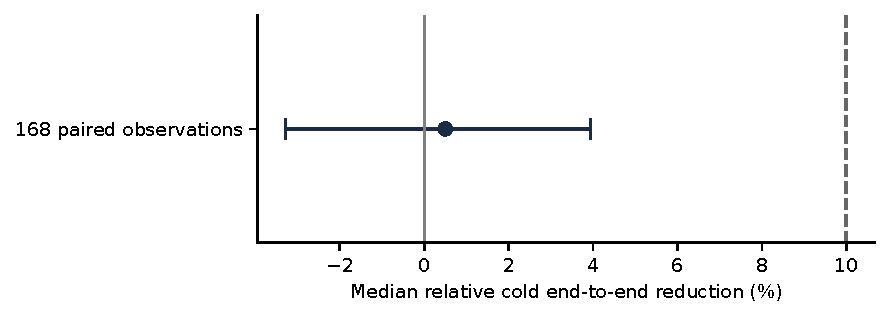
\includegraphics[width=.94\textwidth]{figures/original-effect.pdf}
\caption{Original held-out timing estimate with its stored 95 percent seed-cluster confidence interval and registered ten percent reference. The interval crosses zero; neither interval nor population is recomputed for this figure.}\label{fig:original-effect}
\end{figure}


Figure~\ref{fig:scalar-objective} relates the original scalar objective
to the actual returned method optima. Agreement outside the preferred
interval is consistent with the declared finite departure price.
The analytic curve is an evaluation of stored coefficients, not
another timed trial. Figure~\ref{fig:cold-times} instead displays
stored cell medians and interquartile ranges in one asymmetric-elastic
slice. It shows concrete complete-call costs while retaining its
descriptive status. Formulation size and a selected timing curve
cannot establish a general factorization or algorithmic advantage.
\begin{figure}[htbp]\centering
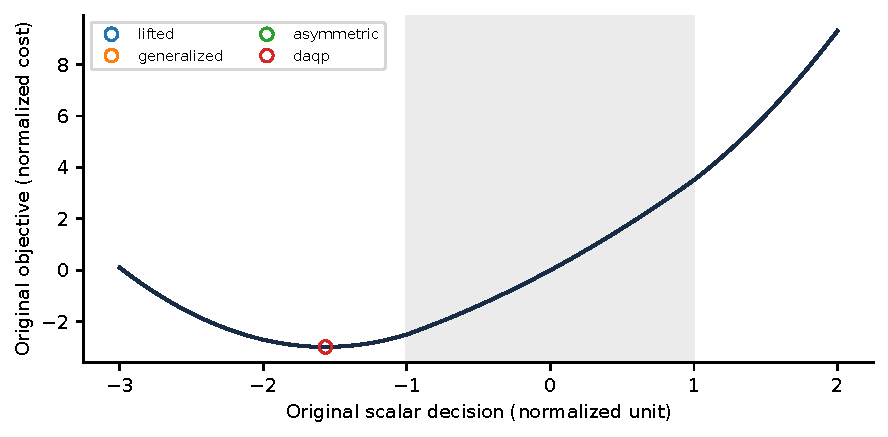
\includegraphics[width=.94\textwidth]{figures/scalar-objective.pdf}
\caption{Analytic evaluation of the stored C01 objective and actual exported method optima. The shaded interval is the preferred band, and the curve is a mathematical illustration rather than a new timed observation.}\label{fig:scalar-objective}
\end{figure}

\begin{figure}[htbp]\centering
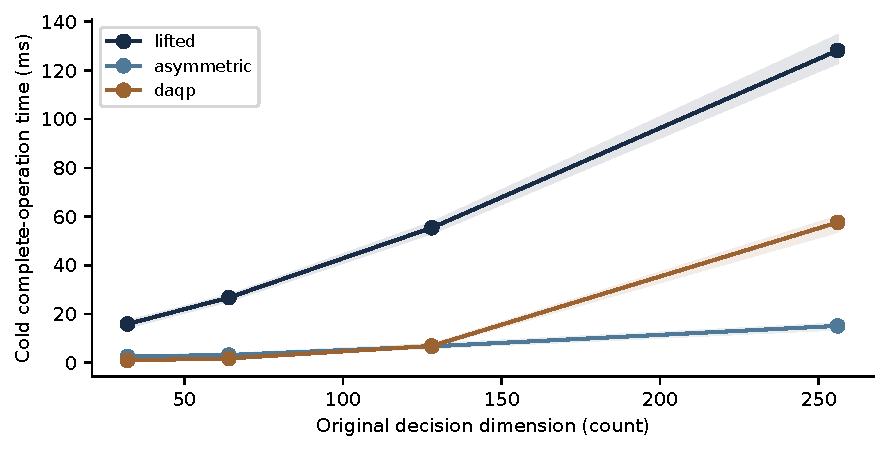
\includegraphics[width=.94\textwidth]{figures/cold-times.pdf}
\caption{Stored held-out asymmetric-elastic timing cells at density 0.05 and unit diagonal condition. Lines are stored medians and bands stored interquartile ranges; this descriptive subset does not replace the complete primary endpoint.}\label{fig:cold-times}
\end{figure}


The original conditioning comparison in
Figure~\ref{fig:conditioning} retains the maximum accepted objective
discrepancy for each compatible robustness cell. The finite grid
extends through diagonal condition$10^6$ without violating the
registered objective/hard limits in admitted observations. This is
not a proof for every near-dependent or arbitrarily scaled problem.
The common-trajectory stream in Figure~\ref{fig:stream-reuse} shows
stored cold and warm durations; it has one observation per frame
and does not support an independent statistical superiority claim.
Its component interpretation is examined in the next section.
\begin{figure}[htbp]\centering
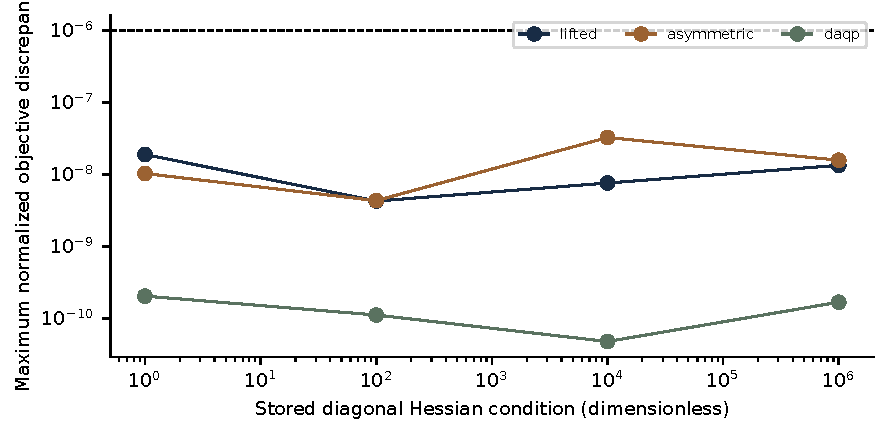
\includegraphics[width=.94\textwidth]{figures/conditioning.pdf}
\caption{Maximum stored objective discrepancy in each compatible robustness cell by diagonal condition. The dashed line is the original external objective criterion; absent methods remain absent rather than receiving an invented zero discrepancy.}\label{fig:conditioning}
\end{figure}

\begin{figure}[htbp]\centering
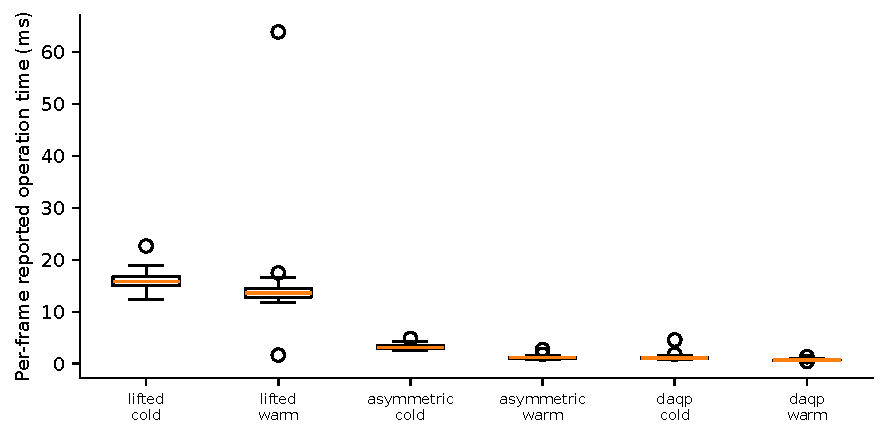
\includegraphics[width=.94\textwidth]{figures/stream-reuse.pdf}
\caption{Stored cold and warm C12 operation durations for every accepted frame of each compatible method. The box summaries are descriptive paired-path evidence, not a randomized causal isolation of warm starting from all other implementation choices.}\label{fig:stream-reuse}
\end{figure}


The grouped study completed all 210 canonical inputs. Its 5670 measured
method observations comprise 3667 accepted,12 accuracy-rejected,
1719 incompatible,270 dependent oracle-failed and two supervised
timeouts. Table~\ref{tab:coupled-states} and
Figure~\ref{fig:coupled-states} retain those categories separately
in development, held-out and robustness splits. The 7770 raw
observations additionally retain warm-ups and oracle calls. All
163390 returned candidate frames satisfy the applicable original-
space checks;44 noncandidate backend-limit frames remain distinct.
Framewise mathematical agreement does not override a failed operation's
batch-level state or the primary failed-pair treatment.
\begin{table}[htbp]\centering\footnotesize
\caption{Measured grouped-study method states by split, including dependent oracle failures and supervised timeouts. Counts cover all measured method rows, while warm-up and oracle observations remain in the larger raw archive.}\label{tab:coupled-states}
\begin{tabularx}{\textwidth}{@{}>{\raggedright\arraybackslash}Xrrrrr@{}}\toprule
Split & Accepted & Accuracy & Incompat. & Oracle & Timeout\\\midrule
development & 879 & 0 & 396 & 21 & 0\\
heldout & 2587 & 6 & 1188 & 105 & 2\\
robustness & 201 & 6 & 135 & 144 & 0\\
\bottomrule\end{tabularx}
\end{table}

\begin{figure}[htbp]\centering
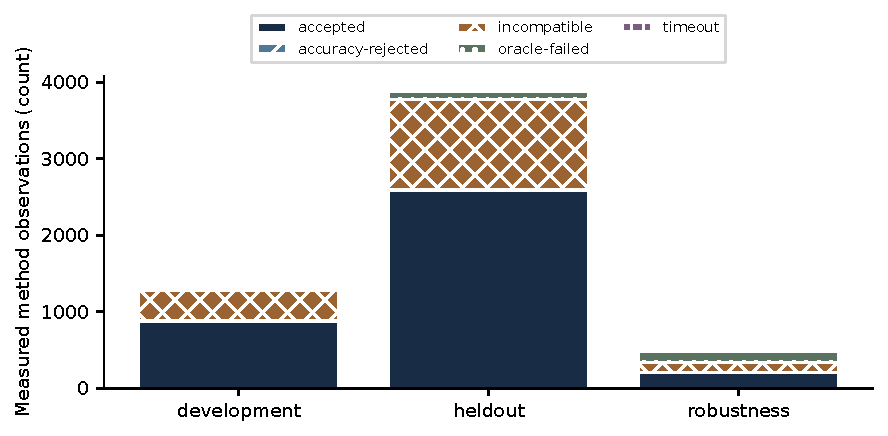
\includegraphics[width=.94\textwidth]{figures/coupled-states.pdf}
\caption{All 5670 measured method observations of the grouped study, separated by their original development, held-out and robustness splits. Acceptance, accuracy rejection, incompatibility, dependent oracle failure and supervised timeout remain different categories.}\label{fig:coupled-states}
\end{figure}


The complete 144-member grouped endpoint is shown in
Figure~\ref{fig:coupled-population}. Nine failed pairs retain their
prespecified score; six missing native medians remain gaps. No
reference is selected where the primary rule selected none.
The median paired score is \PrimaryEstimate\%, with 95\% limits
\PrimaryLower\% and \PrimaryUpper\%. These percentages do not
describe a uniform slowdown of every instance, and the result
does not become favorable by discarding unsuccessful members.
Figure~\ref{fig:coupled-formulations} shows returned per-instance
method medians with their differing sample counts. Those unmatched
distributions characterize concrete formulations but are not an
alternative primary estimator.
\begin{figure}[htbp]\centering
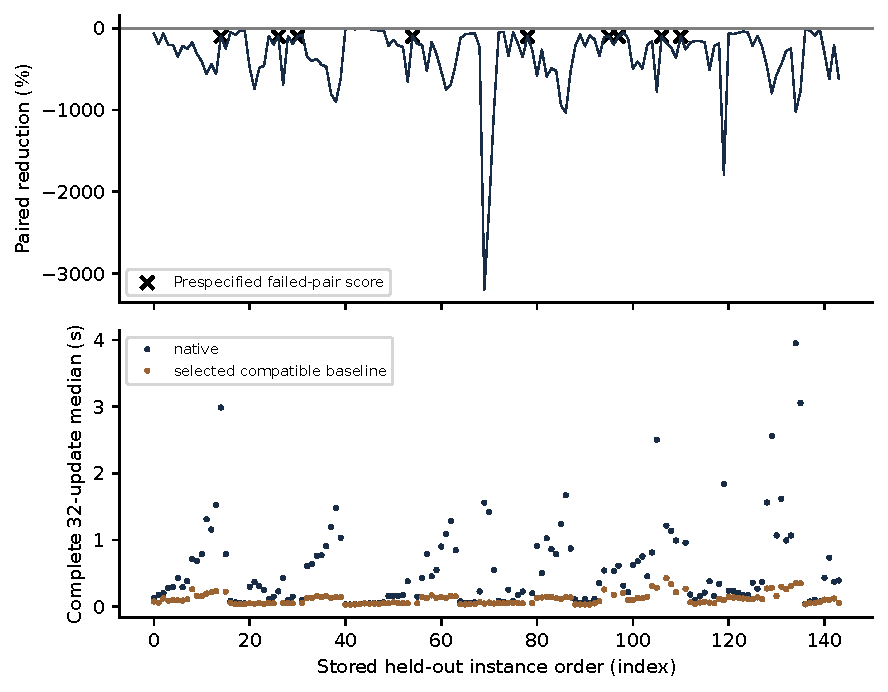
\includegraphics[width=.94\textwidth]{figures/coupled-population.pdf}
\caption{All 144 stored grouped-study primary members in original order, with nine failed scores retained. Complete-operation medians preserve missing values as gaps and do not impute a comparator where the primary rule selected none.}\label{fig:coupled-population}
\end{figure}

\begin{figure}[htbp]\centering
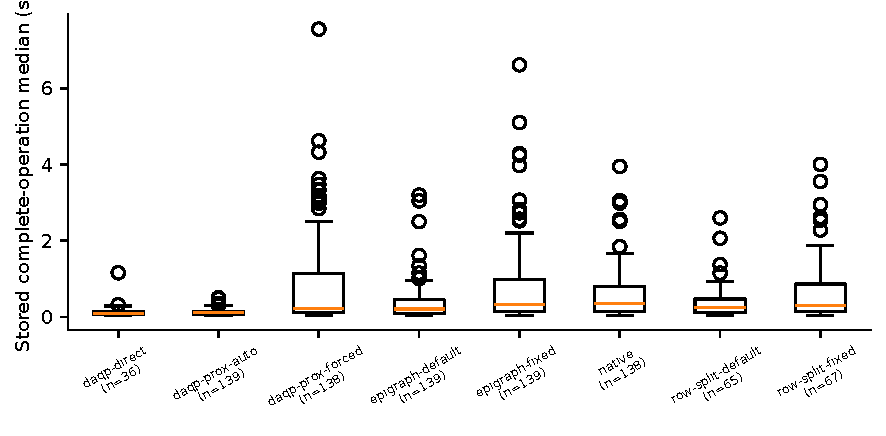
\includegraphics[width=.94\textwidth]{figures/coupled-formulations.pdf}
\caption{Distributions of stored held-out per-instance medians for each returned compatible formulation. Sample counts differ because compatibility and failures differ; these unmatched descriptive distributions are not the registered paired comparison or a causal ablation.}\label{fig:coupled-formulations}
\end{figure}


Figure~\ref{fig:directional-lesson} supplies a transparent original-
space agreement example from the stored physical teaching input.
Native, compact-epigraph and directional row-split answers agree
on objective and decision within their numerical criteria. The
example supports the intended formulation equivalence; it adds
no timed observation to either registered population. Its role
is to separate a mathematical or implementation correctness claim
from the computational hypothesis that the full studies refute.
Thus the results are consistent: exact proximal identities and
small accepted examples coexist with negative complete-operation
timing findings on the specified tested populations.
\begin{figure}[htbp]\centering
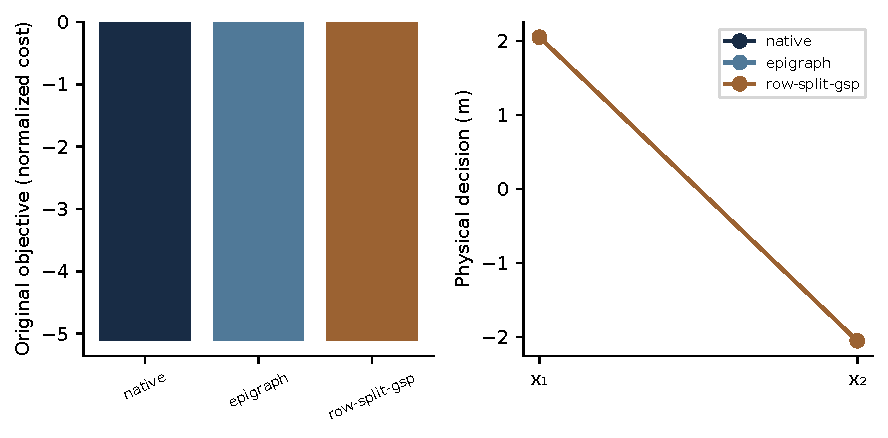
\includegraphics[width=.94\textwidth]{figures/directional-lesson.pdf}
\caption{Stored native, epigraph and directional row-split answers for the same two-variable physical teaching input. Objective and decision agreement are a small numerical illustration, not additional timing evidence or an independent experiment.}\label{fig:directional-lesson}
\end{figure}

The twelve accuracy-rejected batches include backend or iteration-limit
and absent-vector outcomes, rather than twelve returned vectors failing
the independent KKT calculation. Six held-out row-split batches returned
status seven without a candidate vector. Native and forced-proximal DAQP
operations account for the two timeouts. Six robustness oracle limits
leave 144 dependent measured rows with oracle-failed state in that split.
Those dependency counts are distinct from the nine failed primary pairs.
All returned candidate frames passed their applicable original-space
checks; a batch-level backend status remains a separate acceptance condition.

\section{Ablation and retained component comparisons}\label{sec:ablation}
A causal ablation would intervene on one implementation feature
while preserving the same problem, inputs, acceptance criteria and
other numerical choices. The retained evidence does not perform
every such intervention. Table~\ref{tab:ablation} instead states
which component comparisons actually exist and what they can
support. This distinction prevents a required analysis section
from being filled with an invented experiment or an unsupported
causal explanation for the primary timing outcome.

\begin{table}[htbp]\centering\small
\caption{Scope of retained component comparisons and unperformed causal interventions. Each row distinguishes recorded numerical evidence from a stronger attribution that the existing experimental design does not establish.}\label{tab:ablation}
\begin{tabularx}{\textwidth}{@{}lXX@{}}\toprule
Component & Existing comparison & Inference limit\\\midrule
Representation & Native, compact epigraph and row-split policies & Complete policies differ; no isolated causal factorization effect\\
Workspace reuse & Common C12 cold/warm observations & No independent intervention on every initial iterate, cache and active set\\
Conditioning & Fixed-within-seed diagonal condition sweep & Finite robustness grid, not arbitrary physical scaling\\
Directional policy & Same-input equivalent teaching formulations & Correctness illustration, not timed performance or field benefit\\
Threshold implementation & Native exact prefix operation & No alternative sorting implementation timed in isolation\\
Acceptance overhead & Included original-space checks & No post-hoc removal to improve the registered endpoint\\\bottomrule
\end{tabularx}
\end{table}

The formulation comparison retains exact objectives. Row splitting
changes row count and scaling while using a published grouped
projection backend; a compact epigraph changes variable structure
and can interact differently with sparse ordering and numerical
preparation. The returned time distributions therefore compare
complete reference policies. They do not isolate one matrix-size
effect or prove that a threshold sort explains every difference.
The unequal compatibility and failure counts in
Figure~\ref{fig:coupled-formulations} further prevent reading its
unmatched boxes as a causal ranking on one common successful subset.

Cold/warm reuse provides a different component view. All methods
receive the same oracle-driven C12 states, so differences are not
caused by independently divergent plant trajectories. However,
warm mode may retain factors, active sets and iterates together,
while setup accounting also changes. The stream has one observation
per frame and remains descriptive. It cannot assign the entire
reduction to any one retained object or supply the primary
confidence interval. Online active-set literature already uses
parametric structure~\cite{qpOASES}; the observation is not evidence
that reuse was introduced by this implementation.

The conditioning sweep changes diagonal curvature within its
registered seed controls. It supports a bounded statement about
objective/hard-error behavior on that grid. The dimensional
teaching checks test a different invariant: reciprocal row and
directional-scale conversion should preserve physical meaning.
Changing a directional scale alone changes the objective's
allocation policy. Neither comparison is a substitute for an
unperformed randomized intervention on threshold arithmetic or
for a new registered timing study. The fixed primary outcomes
therefore remain the inferential conclusions, while these
component analyses explain what future mechanism-specific
experiments would need to hold constant.

\section{Discussion}\label{sec:discussion}
The central result is the coexistence of exact local mathematics
and negative complete-operation timing evidence. The original-row
updates preserve selected formulations without explicit departure
variables in the principal system. That algebraic property is
verified by independent equivalent formulations and original-space
checks. The registered experiments nevertheless fail to establish
their proposed timing gains. There is no contradiction: a smaller
principal representation is only one contributor to preparation,
iteration, recovery and validation cost.

The grouped operation adds a sorted threshold and joint dual
checks. A sparse reference may benefit from simple diagonal
auxiliaries or effective symbolic ordering. A prepared active-set
backend may exploit vector updates efficiently. Dense/sparse
conversion and language-level overhead can also matter. Without
separate controlled instrumentation, these are plausible mechanisms
to investigate rather than measured causal decompositions of the
observed difference. Numerical optimization and floating-point
analysis caution against inferring cost or accuracy from dimension
alone~\cite{nocedal,higham}.

Including the strongest compatible formulations is therefore
important. A symmetric grouped projection backend after directional
row splitting can solve the same directional objective. An epigraph
can represent the same group price with one auxiliary per group.
The computational comparison would be weaker if it omitted either
because its representation differs from the candidate. Similarly,
DAQP's existing side weights prevent an unequal-cost example from
supporting a new expressibility claim. Prior orthant and weighted
projection work constrains the interpretation of the analytic
construction as well as its implementation~\cite{orthant,weighted}.

Operational interpretation requires another separation. A finite
price can intentionally purchase an interval departure. Numerical
optimality does not prove that the chosen price reflects a real
engineering risk or that the resulting physical policy is safe.
Predictive control relies on model, constraints and closed-loop
assumptions beyond solving one convex subproblem~\cite{mayne,rawlings}.
The source-faithful and authored building examples are synthetic,
and the repeated forecasts are not measured building savings.
Their value here is transparent interpretation and repeatable
numerical comparison, not a field-performance claim.

The negative results constrain subsequent research. A revised
method should identify a genuinely different computational
mechanism, state why the strongest reference might fail to
exploit it, and fix a prospective population before measurement.
Selecting favorable current instances, weakening the oracle,
removing acceptance work or changing the failed-pair rule would
answer another question. The complete retained outcomes instead
make it possible to formulate that next question without
misrepresenting either study's original evidence.

Within the stated domain, the proximal formulas remain useful
tools for modeling and independent verification. Their explicit
zero-price, endpoint, sign and metric conditions clarify when
an implementation is solving the intended problem. The present
evidence supports those restricted mathematical and computational
statements. It supplies no global priority claim, general runtime
superiority or guarantee of practical benefit outside the tested
synthetic regimes.

\section{Limitations}\label{sec:limitations}
Internal validity depends on exact objective matching and complete
timing boundaries. The two protocols use different native
profiles, repetitions, populations and operation scopes. Their
primary percentages cannot be pooled or compared as though
they measured the same unit of work. The original 168 paired
observations include repeated measurements of 24 problems;
the grouped primary contains 144 distinct held-out instances.
Both confidence procedures have only six seed clusters.
Cluster resampling preserves a selected dependence structure,
but small-cluster uncertainty can remain substantial~\cite{cameron}.

External validity is limited to the synthetic models and one
nonreserved execution host. Fixed seeds and a supervised process
do not eliminate operating-system interference, thermal behavior,
library maturity or differences between Python/SciPy and native
implementations. The tested sparse dimensions, curvature patterns,
thermal horizons and directional groups do not sample every
industrial QP. The models contain no measured customer data,
field identification uncertainty or operational deployment
evaluation. A negative result in this population is not proof
that original-row updates cannot help another prospectively
defined regime.

Construct validity requires keeping formulation, correctness and
speed separate. Exact objective agreement does not establish
an algorithmic advantage, while a purchased soft departure does
not establish physical failure when that departure is the stated
optimization policy. Conversely, a relaxed feasible representation
does not certify satisfaction of original immutable inequalities.
The reported objectives use model-specific normalized or physical
cost conventions; they cannot be compared across unrelated
cases as realized business benefit.

The theoretical domain is deliberately restricted. Box residual
elimination requires contraction behavior; the proximal identity
uses a fixed positive diagonal metric. The native grouped
interface has disjoint groups and positive finite scales.
The convergence interpretation assumes a saddle point and
admissible fixed relaxation. Dense metrics, overlapping groups,
nonconvex prices and arbitrary adaptive schedules are outside
the proved scope. Finite tests and local arithmetic safeguards
do not constitute a universal finite-precision error theorem.

Finally, the component analysis retains existing comparisons
instead of fabricating a full causal ablation. No independent
sorting implementation or post-hoc removal of acceptance work
was timed. Learned FlexQP parameters were unavailable, so the
fixed reconstruction is not a learned-policy reproduction.
These limits are part of the evidence interpretation and
remain visible alongside the complete failed primary criteria.

\section{Reproducibility}\label{sec:reproducibility}
The public product source is
\url{https://github.com/fsantibanezleal/CAOS_SoftQP}, with native code
in the separate
\url{https://github.com/fsantibanezleal/CAOS_SoftQP_Engine} repository.
The original computation retains its exact historical source
identity; the grouped computation retains its registered source,
protocol and public SDK profile. These identities must not be
replaced by a later wheel merely because the method name matches.

The complete grouped-study evidence is archived at
\url{https://doi.org/10.5281/zenodo.23875194}. The product evidence tree is % voice-ok: cited supporting dataset identity, not this document's deposit narrative
\url{https://github.com/fsantibanezleal/CAOS_SoftQP/tree/2d3f299d80edad49c2599e61bb6e3c875c119043}.
Its \path{data/derived/experiments/campaign.json} and % voice-ok: literal public evidence filename
\path{data/derived/experiments/stream.json} contain the original exported
summaries and common trajectory, while
\path{manuscripts/coupled-peak-study/results/summary/summary.json} contains
the grouped summary. The original native engine source is
\path{d0c69ed974d577ba02adbd4806332270d9425651}; the grouped registered
implementation source is \path{246bf87e690f4d010494c556e2021d311d587422}.
The archive preserves the latter study's protocol and complete unsuccessful
and successful observations, rather than only the displayed primary statistic.

The archived inputs include synthetic generators or canonical
batches, seeds, full observations, unsuccessful states, method
settings, source/environment identities and replay checks.
The manuscript asset generator reads immutable stored objects
and writes vector figures, literal tables and a source digest
manifest. It performs no numerical solve, timing rerun or
bootstrap recomputation. The separate native build command
uses LaTeX and BibTeX and refuses unresolved or clipped output.
Source, mathematical and rendered-page review are distinct
from successful compilation.

Replaying the preserved scientific evidence and rebuilding the
figures does not require private operational data or API
credentials. A fresh timing reproduction requires the exact
registered historical source/environment and a new external
output location; it must not overwrite the original evidence.
The physical teaching exchange is an additional transparent
illustration and contributes no observations to either
registered primary population.

\paragraph{Declaration of generative AI use.}
Generative AI tools assisted source synthesis, mathematical
checking, implementation and drafting. Numerical and editorial
claims were checked against independent formulations and
preserved computational evidence. Responsibility for the work
rests with the named author.

\section{Conclusions}\label{sec:conclusions}
Side-specific interval and directional disjoint-group penalties
admit explicit original-row proximal calculations in the stated
positive diagonal-metric setting. The box-contraction argument,
scalar threshold and joint dual budget identify the mathematical
conditions needed to recover the intended original objective.
Equivalent lifting, directional row splitting and compact
epigraphs delimit the claim: these objectives were already
expressible, and no priority assertion follows from retaining
the original principal rows.

The completed computational predictions are negative. The
original 456-instance study has a primary 168-observation median
reduction of \OriginalEstimate\%, with 95\% limits \OriginalLower\%
and \OriginalUpper\%. The separate grouped 210-instance study
has a 144-member primary score of \PrimaryEstimate\%, limits
\PrimaryLower\% and \PrimaryUpper\%, and \PrimaryFailed{} retained
failed pairs. Neither establishes the registered 10\% gain.

Correct local mathematics and original-space agreement therefore
do not by themselves establish a faster complete numerical
operation. Future computational work should target a specific
new mechanism and evaluate it prospectively against the strongest
compatible references. The present findings support restricted
derivations, reproducible implementation analysis and complete
negative evidence; they do not establish operational safety,
field benefit or general solver superiority.

\bibliographystyle{plain}
\bibliography{references}
\end{document}
